%--------Desarrollo de la Biblioteca
%--------Daniel Ochoa John
%--------05/06/2012
\chapter{Desarrollo de la biblioteca}
\label{cap:desarrollo}

En este capítulo se presenta el desarrollo de la biblioteca que este trabajo propone, según la metodología OMT++ simplificada. Este capítulo será dividido en distintas secciones, donde cada una de ellas refleja el proceso realizado durante cada fase de esta metodología: análisis, diseño y desarrollo de la solución.

\section{Captura de requerimientos}
Como se mencionó anteriormente, en esta sección se expresarán los conceptos y consideraciones respectivas a la fase de captura de requerimientos. Se describirán los requisitos funcionales y no funcionales obtenidos. Por último, se definirá al actor del sistema.

\subsection{Fundamentos de la soluci\'on}

Este trabajo tiene como principal objetivo el desarrollo de una biblioteca que permita obtener, desde \textit{Facebook} y \textit{Twitter}, los contactos con los que una persona interactúa más. Los datos de entrada al sistema serán los documentos XML con la información conseguida desde las Redes Sociales anteriormente mencionadas. Es muy importante señalar, que para la biblioteca desarrollada, el usuario directo no será una persona, sino que será otra aplicación. 

\subsection{Requisitos funcionales}
\label{functional}
Se presentan los requisitos funcionales del sistema que fueron considerados para el desarrollo de la solución.

\begin{enumerate}
\item El sistema debe leer el documento XML de entrada correspondiente a \textit{Facebook}. 
\item El sistema debe leer el documento XML de entrada correspondiente a \textit{Twitter}.
\item El sistema debe  soportar la definición de la cantidad de contactos cercanos que se desea obtener como resultado.
\item El sistema debe entregar la información al usuario del sistema, mediante comunicación entre aplicaciones.
\item El sistema debe definir los contactos más cercanos al usuario de Redes Sociales en base a los documentos XML de entrada.
\item El sistema debe soportar como opción exportar los resultados obtenidos en formato XML.
\end{enumerate}

\subsection{Requisitos no funcionales}

Se presentan los requisitos no funcionales del sistema que fueron considerados para el desarrollo de la solución.
\begin{enumerate}
\item El sistema debe ser desarrollado en lenguaje Java.
\item El sistema debe ser una biblioteca, permitiendo su integración por parte de otros sistemas.
\item El sistema debe contemplar sólo a \textit{Facebook} y \textit{Twitter} como Redes Sociales.
\item El sistema debe recibir, como parámetros de entrada, documentos XML que contengan la información del usuario de Redes Sociales.
\item El sistema debe definir el formato del documento XML de salida.
\end{enumerate}

\subsection{Casos de uso}

\subsubsection{Actor del sistema}

Se identificó solamente un tipo de actor externo en el sistema: una aplicación cliente (a partir de ahora, sólo cliente). Este cliente realiza peticiones a la biblioteca con el fin de obtener cierta información. En otras palabras, la biblioteca desarrollada en este trabajo es utilizable por un cliente, el cual está siendo utilizado por una persona. Como el sistema desarrollado es una API, la mayor parte de las operaciones son realizadas por el sistema sin la petición de un actor externo.

\subsubsection{Exposición de los casos de uso}

En este apartado, se expondrán los distintos casos de uso para el sistema desarrollado. Estos se derivan de los requisitos funcionales que ya se han expuesto en la subsección \ref{functional}. Cada caso de uso cuenta con la siguiente información:

\begin{enumerate}
\item Caso de Uso: Nombre del caso de uso.
\item Resumen: Muestra, en líneas generales, la funcionalidad del caso de uso.
\item Actor: Enuncia al actor que participa en el desarrollo del caso de uso.
\item Pre-condiciones: Antecedentes que deben existir para que el caso de uso pueda ser llevado a cabo.
\item Descripción: Muestra la funcionalidad del caso de uso en lenguaje natural, considerando las distintas excepciones que puedan ocurrir.
\item Pos-condiciones: Estado del sistema luego de que el flujo de eventos que el caso de uso describe se ha completado correctamente.
\end{enumerate}

\begin{table}[H]
\begin{center}
\caption[Caso de uso \#1 procesando información externa.]{Caso de uso \#1 procesando información externa.}
\label{tab:des-tab01}
\begin{tabular}{|c|>{\raggedright}p{10cm}|}
\hline 
Caso de uso \#1 & \multicolumn{1}{l|}{Procesando información externa.}\tabularnewline
\hline 
\hline 
Resumen & El sistema lee los documentos XML de entrada correspondientes a \emph{Facebook
y Twitter}, posteriormente procesa la información obtenida en los
documentos antes mencionados con la finalidad de generar los resultados.\tabularnewline
\hline 
Actor & Aplicación cliente.\tabularnewline
\hline 
Precondiciones & \multicolumn{1}{l|}{La existencia de documentos XML de entrada.}\tabularnewline
\hline 
Descripción & El sistema lee los documentos XML de entrada {[}\emph{Excepción nº1:
Uno de los archivos de entrada posee un formato erróneo}{]}, cuyas
rutas {[}\emph{Excepción nº2: Los documentos XML de entrada no existen}{]}
son proporcionadas por el cliente, junto con la cantidad de resultados
que el actor desea obtener. Luego de esto, el sistema hace uso de
la información obtenida desde los documentos XML, para luego unir
contactos similares junto a la información respectiva, localmente
en cada Red Social.\tabularnewline
\hline 
Excepciones & Excepción nº1- Uno de los archivos de entrada posee un formato erróneo:
El sistema detecta que uno de los documentos de entrada al sistema
no cumple con el Schema respectivo. Camino alternativo: El sistema
genera una alerta al usuario respecto de la excepción encontrada,
el actor debe enviar nuevamente los archivos al sistema. Si el problema
persiste, se debe generar los documentos XML nuevamente. \textcompwordmark{}Excepción
nº2 - Los documentos XML de entrada no existen: El sistema no puede
encontrar la ubicación física de los documentos de entrada. Esto puede
ser debido a que la ruta de los archivos, que fue proporcionada por
el actor, es incorrecta o bien, los archivos no existen definitivamente.
Camino alternativo: El sistema genera una alerta al usuario respecto
de la excepción generada, si el problema es ocasionado por un error
en las rutas de los archivos, el actor debe reiniciar el proceso utilizando
las rutas correctas.\tabularnewline
\hline 
Pos-condiciones & El sistema queda habilitado para que el actor pueda usar los casos
de uso \#2,\#3 y \#4.\tabularnewline
\hline 
\end{tabular}
\end{center}
\end{table}


\begin{table}[H]
\begin{center}
\caption[Caso de uso \#2 exportando resultados en formato XML.]{Caso de uso \#2 exportando resultados en formato XML.}
\label{tab:des-tab02}
\begin{tabular}{|l|>{\raggedright}p{10cm}|}
\hline 
Caso de Uso \#2 & Exportando resultados en formato XML.\tabularnewline
\hline 
\hline 
Resumen & Cuando el actor lo solicita, el sistema crea un documento XML con
la información asociada a los resultados obtenidos.\tabularnewline
\hline 
Actor & Aplicación cliente.\tabularnewline
\hline 
Pre-condiciones & El actor y el sistema deben haber realizado exitosamente el caso de
uso \#1.\tabularnewline
\hline 
Descripción & El actor solicita al sistema que genere un documento XML con la información
asociada a los resultados obtenidos. El sistema escribe el documento
XML generado en el directorio raíz {[}Excepción mº1: El directorio
raíz está protegido contra escritura.{]} de la aplicación cliente.\tabularnewline
\hline 
Excepciones & Excepcion nº1- El directorio raz esta protegido contra escritura:
El sistema no puede realizar la escritura del documento XML debido
a que el directorio raz de la aplicacion esta protegido contra escritura.
Camino alternativo: El sistema genera una alerta a la aplicacion cliente,
se\textasciitilde{}nalando esta situacion. El sistema no podra cumplir
la tarea de exportar los resultados mediante un documento XML hasta
que se asignen los permisos de escritura al directorio.\tabularnewline
\hline 
Pos-condiciones & Se ha creado un documento XML en el documento raz del El sistema queda
en el estado previo a la realizacion de este caso de uso.\tabularnewline
\hline 
\end{tabular}
\end{center}
\end{table}



\begin{table}[H]
\begin{center}
\caption[Caso de uso \#3 asignando nueva cantidad de resultados.]{Caso de uso \#3 asignando nueva cantidad de resultados.}
\label{tab:des-tab03}
\begin{tabular}{|l|>{\raggedright}p{10cm}|}
\hline 
Caso de Uso \#3 & Asignando nueva cantidad de resultados.\tabularnewline
\hline 
\hline 
Resumen & El actor puede asignar un nuevo valor a la cantidad de resultados
que el sistema otorga.\tabularnewline
\hline 
Actor & Aplicación cliente.\tabularnewline
\hline 
Pre-condiciones & El actor y el sistema deben haber realizado exitosamente el caso de
uso \#1.\tabularnewline
\hline 
Descripción & El actor solicita al sistema que varíe el número de resultados retornados,
enviando a este un número entero especificando la cantidad de resultados
deseada {[}Excepción nº1: El número de resultados deseados excede
a la cantidad disponible.{]}.\tabularnewline
\hline 
Excepciones & Excepción nº1: El número de resultados deseados excede a la cantidad
disponible: El número de resultados solicitados por el actor es más
grande que el total de resultados disponibles. Cuando esto sucede,
el sistema retorna el máximo de resultados posibles al actor.\tabularnewline
\hline 
Pos-condiciones & Se ha variado el número de resultados que el sistema entrega al actor.
El sistema queda en el estado previo a la realizacion de este caso
de uso.\tabularnewline
\hline 
\end{tabular}
\end{center}
\end{table}


\begin{table}[H]
\begin{center}
\caption[Caso de uso \#4 entregando resultados.]{Caso de uso \#4 entregando resultados.}
\label{tab:des-tab04}
\begin{tabular}{|l|>{\raggedright}p{10cm}|}
\hline 
Caso de Uso \#4 & Entregando resultados.\tabularnewline
\hline 
\hline 
Resumen & El sistema entrega los resultados obtenidos luego del procesamiento
de la información entregada.\tabularnewline
\hline 
Actor & Aplicación cliente.\tabularnewline
\hline 
Pre-condiciones & El actor y el sistema deben haber realizado exitosamente el caso de
uso \#1.\tabularnewline
\hline 
Descripción & El actor solicita al sistema los resultados obtenidos luego de realizado
el caso de uso \#1. El sistema entrega los resultados a la aplicación
cliente. La cantidad de resultados que entrega el sistema es la que
ha definido el actor en el caso de uso \#1 o en el caso de uso \#3. \tabularnewline
\hline 
Excepciones & No hay.\tabularnewline
\hline 
Pos-condiciones & El sistema ha entregado los resultados al actor para luego volver
al estado previo a la realización de este caso de uso. \tabularnewline
\hline 
\end{tabular}
\end{center}
\end{table}

\subsection{Diagrama de casos de uso}

Anteriormente se expusieron los distintos casos de uso que tendrá el sistema. En este apartado se mostrará el diagrama de casos de uso respectivo para la aplicación que este trabajo contempla (ver Figura \ref{fig:des-im1}).

\begin{figure}[H]
	\centering
	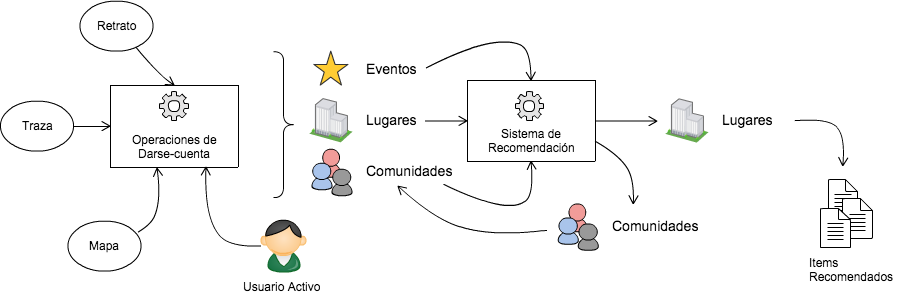
\includegraphics[scale=.15]{images/Figura5-1}
	\caption{\em Diagrama de caso de uso.}
	\label{fig:des-im1}
\end{figure}

\section{Fase de análisis}

La actual sección presenta la descripción del desarrollo de la fase de análisis dispuesta por la metodología. Esta fase permite comprender el sistema a desarrollar, se apoya en los requisitos funcionales y no funcionales.
En las líneas siguientes se mostrará el diccionario de datos, el modelo de objetos y el listado de operaciones que se utilizarán de aquí en adelante.

\subsection{Diccionario de datos}

El diccionario de datos permite presentar en primera instancia a los objetos que se utilizarán en el desarrollo de esta biblioteca. En él se especifican atributos y descripciones, de manera de entregar una herramienta conceptual importante a la hora de comprender el funcionamiento del sistema. La Tabla \ref{tab:des-tab05} muestra el diccionario de datos para este desarrollo.

\begin{table}[H]
\begin{center}
\caption[Diccionario de datos.]{Diccionario de datos.}
\label{tab:des-tab05}
\begin{tabular}{|l|>{\raggedright}p{8cm}|>{\raggedright}p{5cm}|}
\hline 
Nombre de objeto & Descripción de funcionalidad & Atributos\tabularnewline
\hline 
\hline 
FacebookFriend & Este objeto representa a un amigo de \emph{Facebook}. Almacena la
información obtenida desde el documento XML de entrada, o bien la
información obtenida de la unión de contactos similares. & Nombre, ID, Nombre de usuario, Amigos en común, Mensajes en común,
Foto del perfil, Fotos en común, Fecha de cumpleaños, Año de nacimiento,
Género, Tipo de relación. \tabularnewline
\hline 
TwitterFriend & Este objeto representa a un amigo de \emph{Twitter}. Almacena la información
obtenida desde el documento XML de entrada, o bien la información
obtenida de la unión de contactos similares. & Nombre, ID, Nombre de usuario, Foto del perfil, Descripción, Número
de menciones. \tabularnewline
\hline 
MergedFriend & Este objeto representa a un amigo estándar. Se genera cuando se ha
unido la información desde \emph{Twitter} y \emph{Facebook} para un
contacto, o bien cuando se ha demostrado que el contacto es único. & Nombre, FacebookID, TwitterID, Nombre de usuario Facebook, Nombre
de usuario Twitter, Descripción, Foto de perfil en Facebook, Foto
de perfil en Twitter, Género, Fecha de cumpleaños, Grado de relación,
Tipo de relación. \tabularnewline
\hline 
FacebookController & Este objeto representa a un controlador de los amigos de \emph{Facebook}.
Se encarga de las operaciones con este conjunto de datos. & DocumentoXML, ListadeAmigos, XMLSchema.\tabularnewline
\hline 
TwitterController & Este objeto representa a un controlador de los amigos de \emph{Twitter}.
Se encarga de las operaciones con este conjunto de datos. & DocumentoXML, ListadeAmigos, XMLSchema.\tabularnewline
\hline 
MergedController & Este objeto representa al controlador central. Se encarga de crear
la lista con MergedFriend y obtendrá los datos de los controladres
de \emph{Facebook} y \emph{Twitter}. & TwitterController, FacebookController, ListaMerged\tabularnewline
\hline 
Algoritmos & Este objeto estático tendrá todos los algoritmos necesarios para realizar
las operaciones con los datos. & \tabularnewline
\hline 
\end{tabular}
\end{center}
\end{table}

En el apartado siguiente, se procede a generar un diagrama de objetos que permita representar y abstraer los conceptos del domino de este problema. Este modelo es la primera aproximación a la biblioteca propiamente tal.

\subsection{Diagrama de objetos del sistema}

Se presenta a continuación, en la Figura 5-2, el diagrama de objetos del sistema en donde se puede apreciar, en líneas generales, la interacción entre las distintas clases.

\begin{figure}[H]
	\centering
	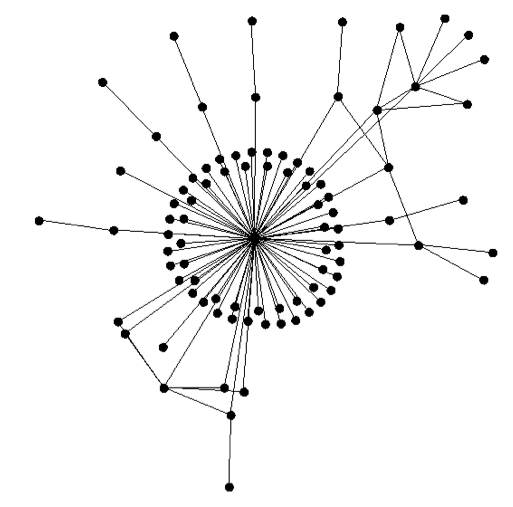
\includegraphics[scale=1]{images/Figura5-2}
	\caption{\em Diagrama de objetos del sistema.}
	\label{fig:des-im2}
\end{figure}

\subsection{Operaciones de la aplicación}

A continuación se muestra la lista de las principales operaciones que puede realizar el usuario con el sistema (ver Tabla \ref{tab:des-tab06}). Estas operaciones fueron concebidas durante la primera etapa del desarrollo de la solución, ya que se derivan de los casos de uso.

\begin{table}[H]
\begin{center}
\caption[Listado de operaciones de la aplicación.]{Listado de operaciones de la aplicación.}
\label{tab:des-tab06}
\begin{tabular}{|l|}
\hline 
Listado de Operaciones\tabularnewline
\hline 
\hline 
A. Leer archivos de entrada.\tabularnewline
\hline 
B. Exportar resultados en formato XML.\tabularnewline
\hline 
C. Asignar la cantidad de resultados.\tabularnewline
\hline 
D. Procesar la información.\tabularnewline
\hline 
E. Entregar resultados.\tabularnewline
\hline 
\end{tabular}
\end{center}
\end{table}

\subsection{Especificación de operaciones}

En esta sección se definen las operaciones anteriormente mencionadas para especificar en forma clara en qué consisten, qué se necesita para llevarlas a cabo y qué sucede una vez que se han realizado. Este proceso se muestra, concretamente, en las tablas siguientes.

\begin{table}[H]
\begin{center}
\caption[Operación leer archivos de entrada.]{Operación leer archivos de entrada.}
\label{tab:des-tab07}
\begin{tabular}{|l|>{\raggedright}p{5cm}|}
\hline 
\multicolumn{2}{|c|}{Especificación de la operación A}\tabularnewline
\hline 
\hline 
\multicolumn{2}{|>{\raggedright}p{8cm}|}{Ilustra el proceso de lectura de los archivos de entrada.}\tabularnewline
\hline 
Operación: & Leyendo archivos de entrada.\tabularnewline
\hline 
Pre-condiciones: & No existen pre-condiciones.\tabularnewline
\hline 
Excepciones: & Los archivos de entrada no existen: Se genera un mecanismo de alerta.
Los archivos de entrada o uno de ellos no tienen un formato correcto:
Se genera un mecanismo de alerta.\tabularnewline
\hline 
Post-condiciones: & El usuario puede realizar la operación B.\tabularnewline
\hline 
\end{tabular}
\end{center}
\end{table}

\begin{table}[H]
\begin{center}
\caption[Operación procesar la información.]{Operación procesar la información.}
\label{tab:des-tab08}
\begin{tabular}{|l|>{\raggedright}p{5cm}|}
\hline 
\multicolumn{2}{|c|}{Especificación de la operación B}\tabularnewline
\hline 
\hline 
\multicolumn{2}{|>{\raggedright}p{8cm}|}{Ilustra el proceso de procesar la información.}\tabularnewline
\hline 
Operación: & Procesando la información.\tabularnewline
\hline 
Pre-condiciones: & El sistema debe haber completado con éxito la operación A.\tabularnewline
\hline 
Excepciones: & No existen excepciones.\tabularnewline
\hline 
Post-condiciones: & El usuario puede realizar las operaciones C, D y E.\tabularnewline
\hline 
\end{tabular}
\end{center}
\end{table}

\begin{table}[H]
\begin{center}
\caption[Operación exportar los resultados en formato XML.]{Operación exportar los resultados en formato XML.}
\label{tab:des-tab09}
\begin{tabular}{|l|>{\raggedright}p{5cm}|}
\hline 
\multicolumn{2}{|c|}{Especificación de la operación C}\tabularnewline
\hline 
\hline 
\multicolumn{2}{|>{\raggedright}p{8cm}|}{Ilustra el proceso de exportar los resultados en formato XML.}\tabularnewline
\hline 
Operación: & Exportando resultados en formato XML.\tabularnewline
\hline 
Pre-condiciones: & El sistema debe haber completado con éxito la operación B.\tabularnewline
\hline 
Excepciones: & El directorio de destino está protegido contra escritura: Se genera
un mecanismo de alerta.\tabularnewline
\hline 
Post-condiciones: & El sistema ha exportado los datos en forma de documento XML, para
luego volver al estado obtenido en la operación A.\tabularnewline
\hline 
\end{tabular}
\end{center}
\end{table}

\begin{table}[H]
\begin{center}
\caption[Operación asignar nueva cantidad de resultados.]{Operación asignar nueva cantidad de resultados.}
\label{tab:des-tab10}
\begin{tabular}{|l|>{\raggedright}p{5cm}|}
\hline 
\multicolumn{2}{|c|}{Especificación de la operación D}\tabularnewline
\hline 
\hline 
\multicolumn{2}{|>{\raggedright}p{8cm}|}{Ilustra el proceso de asignación de una nueva cantidad de resultados.}\tabularnewline
\hline 
Operación: & Solicitando nueva cantidad de resultados.\tabularnewline
\hline 
Pre-condiciones: & El sistema debe haber completado con éxito la operación B.\tabularnewline
\hline 
Excepciones: & El número solicitado excede a la cantidad de resultados obtenidos:
Se genera un mecanismo de alerta.\tabularnewline
\hline 
Post-condiciones: & El sistema ha cambiado el número de resultados que retornará. Posteriormente
vuelve al estado obtenido en la operación A.\tabularnewline
\hline 
\end{tabular}
\end{center}
\end{table}

\begin{table}[H]
\begin{center}
\caption[Operación entregar resultados.]{Operación entregar resultados.}
\label{tab:des-tab11}
\begin{tabular}{|l|>{\raggedright}p{5cm}|}
\hline 
\multicolumn{2}{|c|}{Especificación de la operación E}\tabularnewline
\hline 
\hline 
\multicolumn{2}{|>{\raggedright}p{8cm}|}{Ilustra el proceso de entregar los resultados al usuario.}\tabularnewline
\hline 
Operación: & Entregando resultados.\tabularnewline
\hline 
Pre-condiciones: & El sistema debe haber completado con éxito la operación B.\tabularnewline
\hline 
Excepciones: & No existen excepciones.\tabularnewline
\hline 
Post-condiciones: & El sistema ha entregado los resultados a la aplicación cliente. Posteriormente
vuelve al estado obtenido en la operación A.\tabularnewline
\hline 
\end{tabular}
\end{center}
\end{table}

\section{Fase de diseño}

En esta fase se presentará la arquitectura que se ha utilizado en la biblioteca desarrollada en este trabajo, así como también el diagrama de clases respectivo. De manera adicional, se incluyen los diagramas de secuencia. Estos diagramas indican cómo transcurre la acción en la aplicación, mostrando las interacciones que existen entre las distintas clases para lograr la realización de las distintas actividades definidas anteriormente en fase de análisis.

\subsection{Arquitectura de la solución}

La arquitectura que posee la solución comprende un modelo a tres capas que se comunican entre sí. Estas capas están comprendidas por los modelos, los controladores y el módulo de interacción con el cliente.

La capa modelo se encarga de la representación computacional común de los datos obtenidos desde las Redes Sociales, permitiendo un manejo simple de la información almacenada. Esta capa está formada por las siguientes clases:

\begin{list}{•}
\item TwitterFriend: Esta clase se encarga de modelar los datos obtenidos desde \textit{Twitter} para un contacto. Interactúa solamente con el controlador de \textit{Twitter}. 
\item FacebookFriend: Esta clase se encarga de modelar los datos obtenidos desde \textit{Facebook} para un contacto. La interacción que tiene esta clase es solamente con el controlador de \textit{Facebook}.
\item MergedFriend: Esta clase se encarga de modelar los datos que representan a un contacto unido, es decir, cuando se ha encontrado un contacto similar en \textit{Facebook} y \textit{Twitter} la información combinada de ambas fuentes genera un MergedFriend. Solamente interactúa con el controlador \textit{Merged}, los objetos de esta clase son los que se retornan como resultado al cliente.
\end{list}

La capa controlador se encarga de realizar procesos y operaciones con y entre los datos del modelo. Se compone de tres controladores, los cuales son representados por las siguientes clases:

\begin{list}{•}
\item FacebookController: Esta clase representa al controlador para los datos de \textit{Facebook}. Se encarga de crear objetos del modelo en base a la lectura del documento de entrada respectivo, procesar la información y reducir contactos duplicados.
\item TwitterController: Esta clase representa al controlador para los datos de \textit{Twitter}. Se encarga de crear objetos del modelo en base a la lectura del documento de entrada respectivo, procesar la información y reducir contactos duplicados. 
\item MergedController: Esta clase representa al controlador de los datos unidos. Se encarga de unir la información creada por los controladores de \textit{Facebook} y \textit{Twitter}, creando objetos de contactos unidos. Este controlador almacena los resultados obtenidos por la biblioteca y que son, en último término, los que el usuario final obtiene. Con el propósito de acceder a la información contenida en cada controlador, esta clase interactúa directamente con las otras de su capa. Es el controlador principal del sistema.
\end{list}

El módulo de comunicación con la aplicación cliente está representado por la clase SocialNetworkMerger, la cual proporciona al cliente una capa de abstracción de los procesos de la biblioteca permitiendo una comunicación simple. Esta clase se encarga de dirigir las peticiones del cliente a los controladores correspondientes así como también de retornar las respuestas respectivas. Las interacciones mencionadas pueden apreciarse en la Figura 5-3.


\begin{figure}[H]
	\centering
	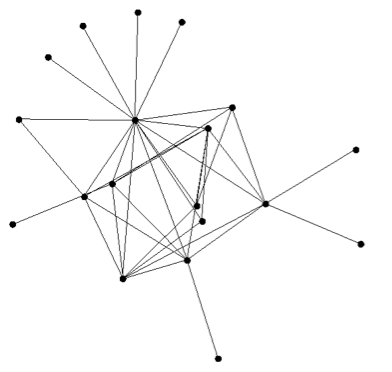
\includegraphics[scale=.7]{images/Figura5-3}
	\caption{\em Interacciones presentes en la biblioteca.}
	\label{fig:des-im3}
\end{figure}

\subsection{Elementos externos incorporados}

Se han incorporado elementos externos a la solución con la finalidad de reutilizar código existente y que permite cumplir con las funcionalidades propuestas para la biblioteca, estos elementos también son bibliotecas o API que están disponibles gratuitamente en la Web. Las API externas incorporadas a la solución son:

\begin{enumerate}
\item String Similarity1.0.0 (Rice, 2011) : Esta API, que cuenta con licencia MIT, permite realizar cálculos de similitud entre cadenas de caracteres según los algoritmos de Jaro-Winkler y el coeficiente de Dice. 
\item JDom 1.1.2 (Hunter \& McLaughlin, 2000) : Esta API, que cuenta con licencia Apache, permite una representación en lenguaje Java de un documento XML, facilitando los procesos de lectura y escritura de éstos.
\item ValidadorXML (Ortiz, 2011) : Esta API distribuida libremente por el autor, permite encapsular el proceso de validación de un documento XML contra el correspondiente Schema.
\end{enumerate}

\subsection{Diagrama de clases}
Se presenta a continuación el diagrama de clases para la fase de diseño. Este diagrama será utilizado en la implementación de la solución y engloba la arquitectura descrita anteriormente, al utilizar controladores y modelos para el tratamiento y procesamiento de la información. En la Figura \ref{fig:des-im4} se puede apreciar el diagrama en su totalidad. 

Para facilitar la lectura del diagrama, se ha incluido cada clase en un tamaño mayor. Las clases se indican en un orden establecido, el cual es, tomando como referencia el diagrama de la Figura \ref{fig:des-im4}, desde izquierda a derecha, de arriba a abajo. Esto comprende desde la Figura 5-5 hasta la Figura 5-13.

\begin{figure}[H]
	\centering
	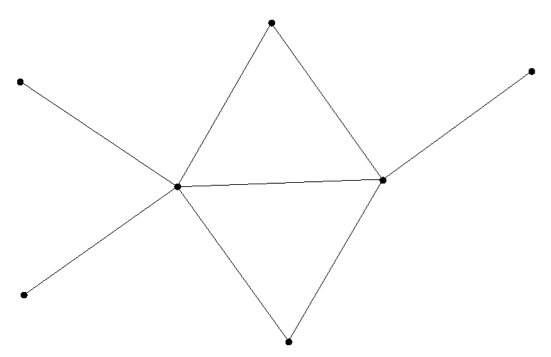
\includegraphics[scale=.4]{images/Figura5-4}
	\caption{\em Diagrama de clases fase de diseño.}
	\label{fig:des-im4}
\end{figure}

\begin{figure}[H]
	\centering
	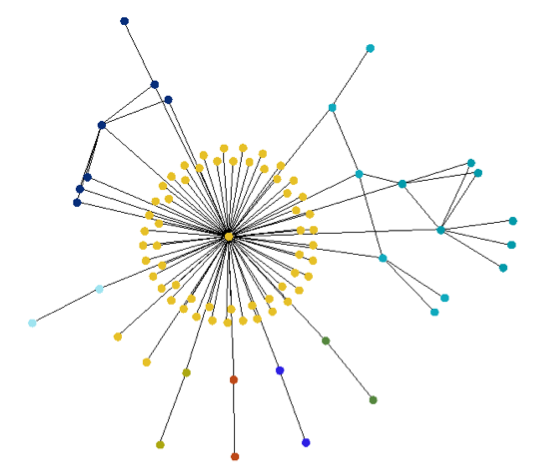
\includegraphics[scale=.4]{images/Figura5-5}
	\caption{\em Clase FacebookFriend.}
	\label{fig:des-im5}
\end{figure}

\begin{figure}[H]
	\centering
	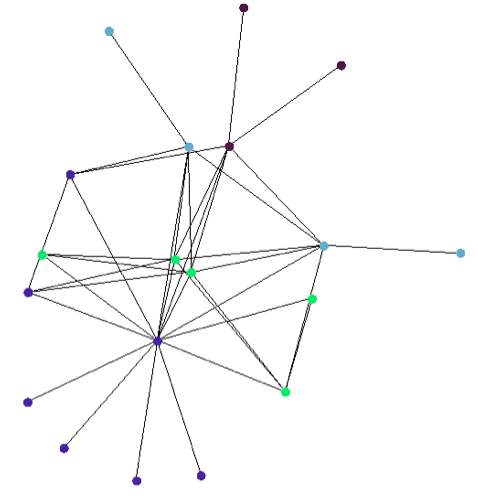
\includegraphics[scale=.4]{images/Figura5-6}
	\caption{\em Clase FacebookController.}
	\label{fig:des-im6}
\end{figure}

\begin{figure}[H]
	\centering
	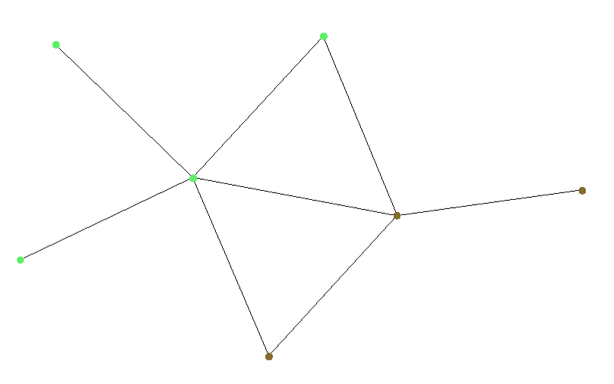
\includegraphics[scale=.4]{images/Figura5-7}
	\caption{\em Clase MergedController.}
	\label{fig:des-im7}
\end{figure}

\begin{figure}[H]
	\centering
	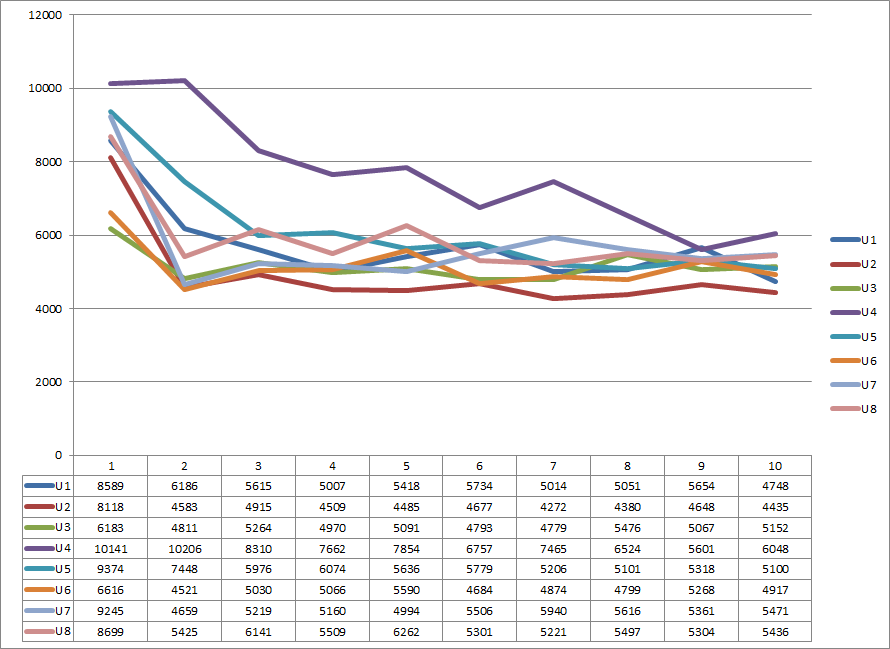
\includegraphics[scale=.4]{images/Figura5-8}
	\caption{\em Clase Bubblesort.}
	\label{fig:des-im8}
\end{figure}

\begin{figure}[H]
	\centering
	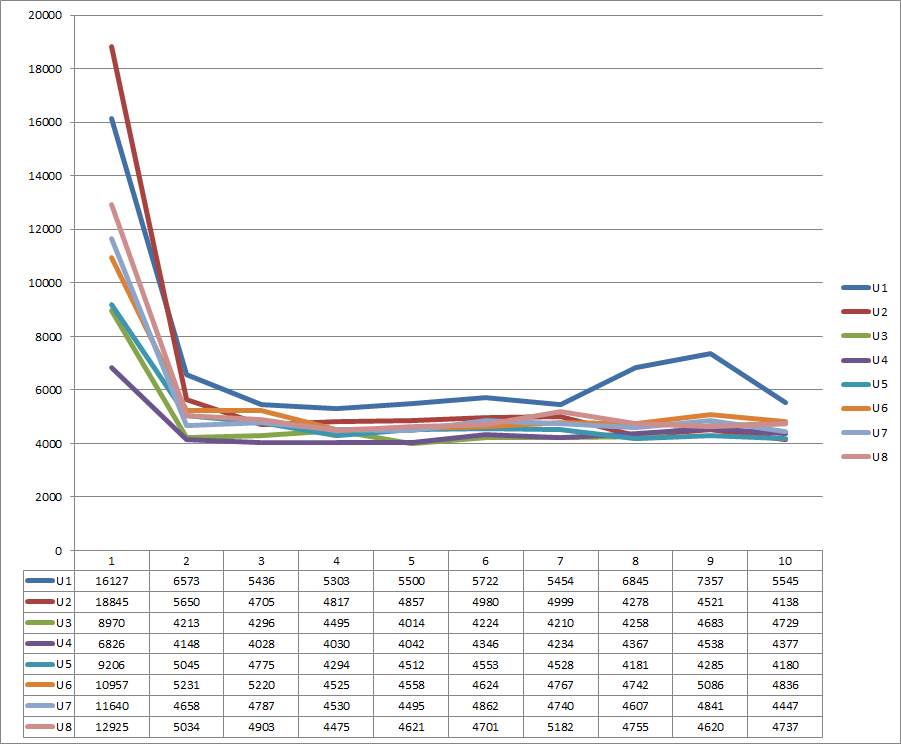
\includegraphics[scale=.4]{images/Figura5-9}
	\caption{\em Clase Comparaciones.}
	\label{fig:des-im9}
\end{figure}

\begin{figure}[H]
	\centering
	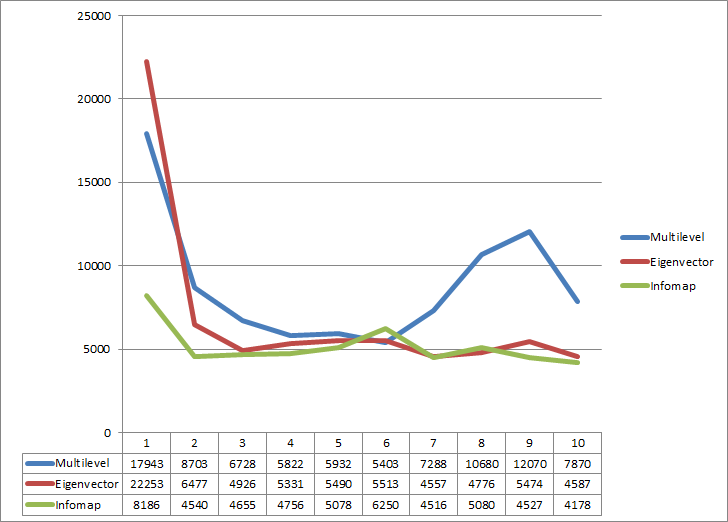
\includegraphics[scale=.4]{images/Figura5-10}
	\caption{\em Clase SocialNetworkMerger.}
	\label{fig:des-im10}
\end{figure}

\begin{figure}[H]
	\centering
	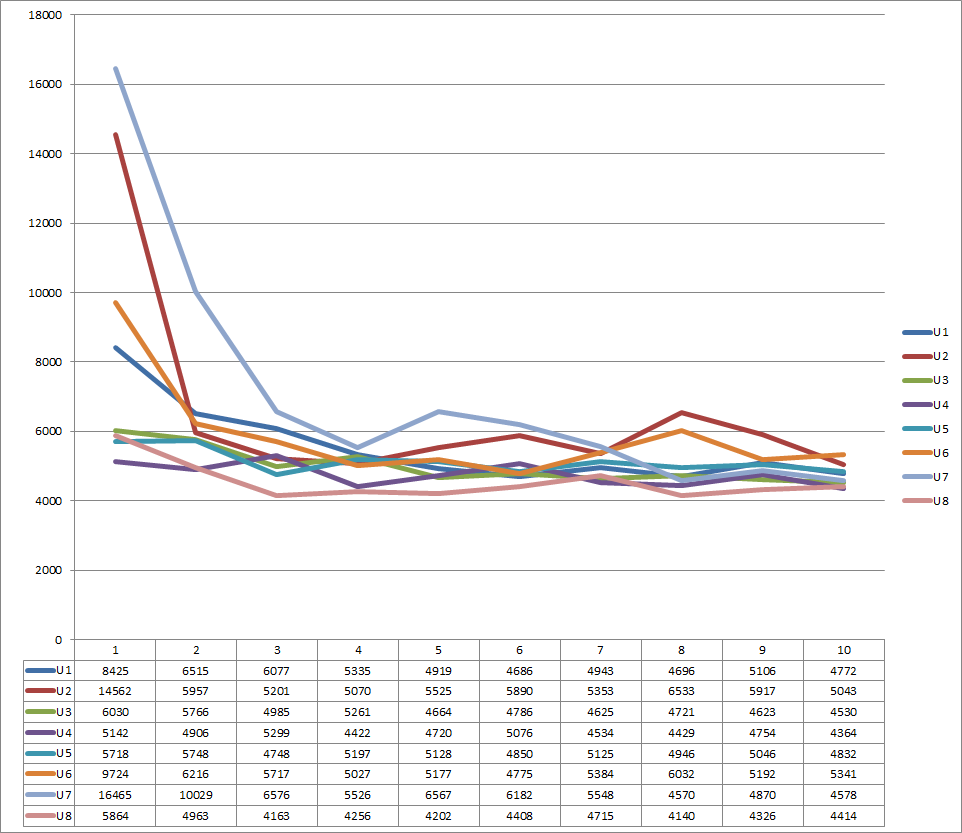
\includegraphics[scale=.4]{images/Figura5-11}
	\caption{\em Clase MergedFriend.}
	\label{fig:des-im11}
\end{figure}

\begin{figure}[H]
	\centering
	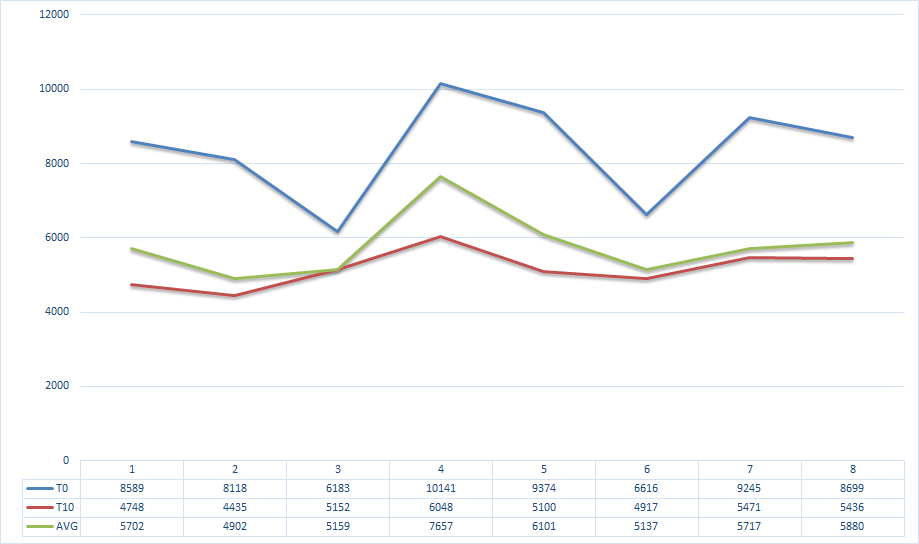
\includegraphics[scale=.4]{images/Figura5-12}
	\caption{\em Clase TwitterController.}
	\label{fig:des-im12}
\end{figure}

\begin{figure}[H]
	\centering
	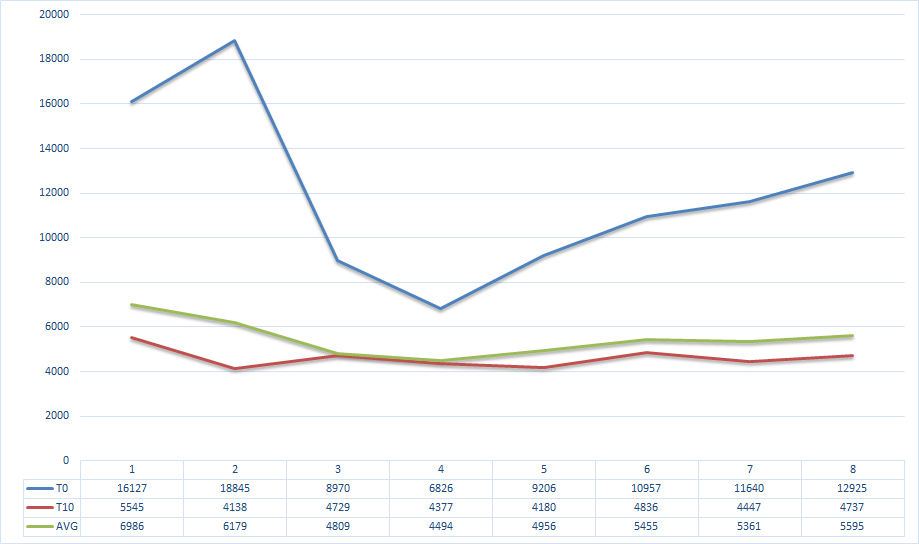
\includegraphics[scale=.4]{images/Figura5-13}
	\caption{\em Clase TwitterFriend.}
	\label{fig:des-im13}
\end{figure}

\subsection{Especificación de clases}

En este apartado se describirá a cada una de las clases anteriormente mostradas mediante el diagrama de clases. Se mostrará, en la Tabla \ref{tab:des-tab23}, el nombre de la clase junto con la descripción de sus funcionalidades. Los atributos y métodos están presentes en el diagrama.

\begin{table}[H]
\begin{center}
\caption[Especificación de clases.]{Especificación de clases.}
\label{tab:des-tab23}
\begin{tabular}{|l|>{\raggedright}p{7cm}|}
\hline 
Clase & Descripción de funcionalidades\tabularnewline
\hline 
\hline 
SocialNetworkMerger & Es la clase principal del sistema. Su función es interactuar con el
usuario, proveyéndole los servicios del sistema. Se comunica con los
controladores \emph{Merged}, \emph{Facebook} y \emph{Twitter} para
obtener y manejar la información.\tabularnewline
\hline 
MergedController & Es el controlador que maneja a los contactos unidos. Contiene los
métodos necesarios para analizar y unir la información obtenida desde
\emph{Facebook }y \emph{Twitter}. Es la clase que realiza la unión
de información entre las Redes Sociales.\tabularnewline
\hline 
FacebookController & Es el controlador que maneja a los contactos obtenidos desde\emph{
Facebook}. Cuenta con todos los métodos para unir y analizar la información
obtenida desde esta Red Social.\tabularnewline
\hline 
TwitterController & Es el controlador que maneja a los contactos obtenidos desde \emph{Twitter}.
Cuenta con todos los métodos para unir y analizar la información obtenida
desde esta Red Social.\tabularnewline
\hline 
MergedFriend & Es una clase que tiene la función de modelar los datos para un contacto
unido, es decir, con la información obtenida desde \emph{Facebook}
y \emph{Twitter}.\tabularnewline
\hline 
FacebookFriend & Es una clase que tiene la función de modelar los datos para un contacto
obtenido desde \emph{Facebook}. \tabularnewline
\hline 
TwitterFriend & Es una clase que tiene la función de modelar los datos para un contacto
obtenido desde \emph{Twitter}.\tabularnewline
\hline 
Comparaciones & Es una clase que contiene métodos que se comunican con la API de\emph{
String Similarity} para comparar los contactos.\tabularnewline
\hline 
BubbleSort & Es una clase que sirve para ordenar los datos mediante algoritmo burbuja.\tabularnewline
\hline 
\end{tabular}
\end{center}
\end{table}

\subsection{Especificación de los diagramas de secuencia}

Se muestra a continuación la especificación correspondiente a los diagramas de secuencia involucrados. En primera instancia, se presentarán las tablas que especifican a los diagramas de secuencias, luego se expondrán los diagramas propiamente tal.

\begin{table}[H]
\begin{center}
\caption[Especificación diagrama de secuencia leer archivo de entrada Facebook.]{Especificación diagrama de secuencia leer archivo de entrada Facebook.}
\label{tab:des-tab13}
\begin{tabular}{|l|>{\raggedright}p{7cm}|}
\hline 
Diagrama de secuencia & Leyendo archivo de entrada \emph{Facebook.}\tabularnewline
\hline 
\hline 
Actor(es): & Usuario.\tabularnewline
\hline 
Resumen: & El actor envía al sistema la dirección física del archivo de entrada
con los datos de \emph{Facebook}. El sistema comprueba que la información
que se está entregando sea válida.\tabularnewline
\hline 
Resultado: & El actor puede solicitar al sistema que comience el procesamiento
de la información.\tabularnewline
\hline 
Excepciones: & 1. Los archivos de entrada no existen o no pueden ser leídos. 

2. Uno o ambos archivos de entrada tienen un formato no válido. \tabularnewline
\hline 
\end{tabular}
\end{center}
\end{table}


\begin{table}[H]
\begin{center}
\caption[Especificación diagrama de secuencia leer archivo de entrada Twitter.]{Especificación diagrama de secuencia leer archivo de entrada Twitter.}
\label{tab:des-tab14}
\begin{tabular}{|l|>{\raggedright}p{7cm}|}
\hline 
Diagrama de secuencia & Leyendo archivo de entrada \emph{Twitter.}\tabularnewline
\hline 
\hline 
Actor(es): & Usuario.\tabularnewline
\hline 
Resumen: & El actor envía al sistema la dirección física del archivo de entrada
con los datos de \emph{Twitter}. El sistema comprueba que la información
que se está entregando sea válida.\tabularnewline
\hline 
Resultado: & El actor puede solicitar al sistema que comience el procesamiento
de la información.\tabularnewline
\hline 
Excepciones: & 1. Los archivos de entrada no existen o no pueden ser leídos. 

2. Uno o ambos archivos de entrada tienen un formato no válido. \tabularnewline
\hline 
\end{tabular}
\end{center}
\end{table}

\begin{table}[H]
\begin{center}
\caption[Especificación diagrama de secuencia procesar la información.]{Especificación diagrama de secuencia procesar la información.}
\label{tab:des-tab15}
\begin{tabular}{|l|>{\raggedright}p{7cm}|}
\hline 
Diagrama de secuencia & Procesando la información.\tabularnewline
\hline 
\hline 
Actor(es): & Usuario.\tabularnewline
\hline 
Resumen: & El actor solicita al sistema procesar la información obtenida desde los archivos de entrada, con la finalidad de generar los resultados respecto a los contactos más cercanos.\tabularnewline
\hline 
Resultado: & El actor puede solicitar al sistema: 
1. Exportar los resultados obtenidos en formato XML. 
2. Entregar los resultados mediante comunicación entre aplicaciones.
3. Reasignar la cantidad de resultados que desea obtener.\tabularnewline
\hline 
Excepciones: & No hay excepciones.\tabularnewline
\hline 
\end{tabular}
\end{center}
\end{table}

\begin{table}[H]
\begin{center}
\caption[Especificación diagrama de secuencia exportar los resultados en formato XML.]{Especificación diagrama de secuencia exportar los resultados en formato XML.}
\label{tab:des-tab16}
\begin{tabular}{|l|>{\raggedright}p{7cm}|}
\hline 
Diagrama de secuencia & Exportando resultados en formato XML.\tabularnewline
\hline 
\hline 
Actor(es): & Usuario.\tabularnewline
\hline 
Resumen: & El actor solicita al sistema que exporte los resultados obtenidos en un documento XML.\tabularnewline
\hline 
Resultado: & El actor obtiene un documento XML con los resultados obtenidos.\tabularnewline
\hline 
Excepciones: & 1. El directorio objetivo está protegido contra escritura .\tabularnewline
\hline 
\end{tabular}
\end{center}
\end{table}

\begin{table}[H]
\begin{center}
\caption[Especificación diagrama de secuencia asignación de la cantidad de resultados.]{Especificación diagrama de secuencia asignación de la cantidad de resultados.}
\label{tab:des-tab17}
\begin{tabular}{|l|>{\raggedright}p{7cm}|}
\hline 
Diagrama de secuencia & Asignando la cantidad de resultados.\tabularnewline
\hline 
\hline 
Actor(es): & Usuario.\tabularnewline
\hline 
Resumen: & El actor asigna al sistema la cantidad de resultados que desea obtener.\tabularnewline
\hline 
Resultado: & El sistema entregará, en la próxima petición de resultados, la cantidad de resultados asignada.\tabularnewline
\hline 
Excepciones: & 1. La cantidad de resultados deseada es mayor que el número de resultados disponibles. El sistema proporciona al usuario el máximo de resultados disponibles.\tabularnewline
\hline 
\end{tabular}
\end{center}
\end{table}

\begin{table}[H]
\begin{center}
\caption[Especificación diagrama de secuencia entregando resultados.]{Especificación diagrama de secuencia entregando resultados.}
\label{tab:des-tab18}
\begin{tabular}{|l|>{\raggedright}p{7cm}|}
\hline 
Diagrama de secuencia & Entregando resultados.\tabularnewline
\hline 
\hline 
Actor(es): & Usuario.\tabularnewline
\hline 
Resumen: & El actor solicita al sistema los resultados obtenidos luego de procesar la información.\tabularnewline
\hline 
Resultado: & El actor obtiene la información que representa a los \textit{k}-contactos más cercanos del usuario.\tabularnewline
\hline 
Excepciones: & No hay excepciones.\tabularnewline
\hline 
\end{tabular}
\end{center}
\end{table}

\subsection{Diagramas de secuencia}

A continuación, se presentan los diagramas de secuencia especificados y descritos en el punto anterior. 

\begin{figure}[H]
	\centering
	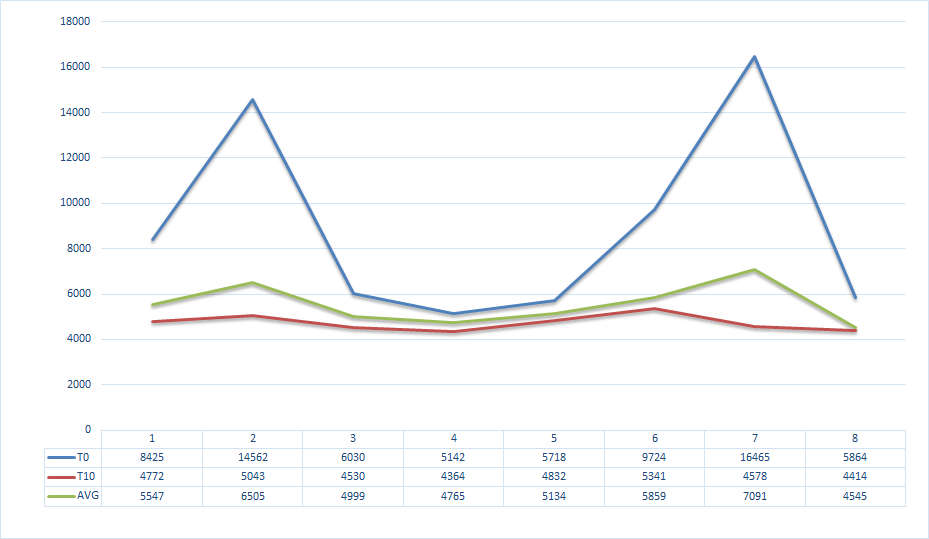
\includegraphics[scale=1]{images/Figura5-14}
	\caption{\em Diagrama de secuencia entregando resultados.}
	\label{fig:des-im14}
\end{figure}

\begin{figure}[H]
	\centering
	\includegraphics[scale=1]{images/Figura5-15}
	\caption{\em Diagrama de secuencia exportando resultados a XML.}
	\label{fig:des-im15}
\end{figure}

\begin{figure}[H]
	\centering
	\includegraphics[scale=1]{images/Figura5-16}
	\caption{\em Diagrama de secuencia asignar cantidad de resultados.}
	\label{fig:des-im16}
\end{figure}

\begin{landscape}
\begin{figure}[H]
	\centering
	\includegraphics[scale=1]{images/Figura5-17}
	\caption{\em Diagrama de secuencia procesar la información.}
	\label{fig:des-im17}
\end{figure}
\end{landscape}

\begin{landscape}
\begin{figure}[H]
	\centering
	\includegraphics[scale=.9]{images/Figura5-18}
	\caption{\em Diagrama de secuencia leer archivo de entrada Facebook.}
	\label{fig:des-im18}
\end{figure}
\end{landscape}

\begin{landscape}
\begin{figure}[H]
	\centering
	\includegraphics[scale=.9]{images/Figura5-19}
	\caption{\em Diagrama de secuencia leer archivo de entrada Twitter.}
	\label{fig:des-im19}
\end{figure}
\end{landscape}